\documentclass[10pt,a4paper,onecolumn]{article}

\usepackage[utf8]{inputenx}
\usepackage[T1]{fontenc}
\usepackage{lmodern}
\usepackage{listings}
\usepackage{textcomp}
\usepackage[english,italian]{babel}
\usepackage{amsmath}
\usepackage{booktabs}
\usepackage{graphicx}
\usepackage[font=small,labelfont=bf,labelsep=period,tableposition=top]{caption}
\usepackage{tabularx}
\usepackage{multirow}
\usepackage{longtable}
\usepackage{fancyhdr}
\usepackage{lastpage}    
\usepackage{color}
\usepackage{enumitem}

\fancyhead{}
\renewcommand{\headrulewidth}{1pt}

\fancyhead[RE,RO]{
\begin{picture}(-135,0)
	\put(-475,0){\sffamily\large\leftmark}
\end{picture}
}

\cfoot{}

\fancyfoot[RO,LE]{\sffamily Pag.~\thepage{} di \pageref{LastPage}} 
\fancyfoot[RE,LO]{RistorESU Nord Piovego}

\renewcommand{\footrulewidth}{.2pt}
\pagestyle{fancy}

\renewcommand{\sectionmark}[1]{\markboth{#1}{#1}} 

% **************************************************
% Cross-references e collegamenti ipertestuali
% **************************************************
\usepackage[]{hyperref}
%\usepackage[hidelinks]{hyperref}
\hypersetup{%
  colorlinks=false, linktocpage=false, pdfborder={0,0,0}, pdfstartpage=1, pdfstartview=FitV,%
  urlcolor=Cyan, linkcolor=Cyan, citecolor=Black, %pagecolor=Black,
  pdfcreator={pdflatex}, pdfproducer={pdflatex with hyperref package}%
}

\definecolor{dkgreen}{rgb}{0,0.6,0}
\definecolor{gray}{rgb}{0.5,0.5,0.5}
\definecolor{mauve}{rgb}{0.58,0,0.82}
 
\lstset{ %
  %language=XHTML,                % the language of the code
  basicstyle=\footnotesize,           % the size of the fonts that are used for the code
  numbers=left,                   % where to put the line-numbers
  numberstyle=\tiny\color{gray},  % the style that is used for the line-numbers
  stepnumber=2,                   % the step between two line-numbers. If it's 1, each line 
                                  % will be numbered
  numbersep=5pt,                  % how far the line-numbers are from the code
  backgroundcolor=\color{white},      % choose the background color. You must add \usepackage{color}
  showspaces=false,               % show spaces adding particular underscores
  showstringspaces=false,         % underline spaces within strings
  showtabs=false,                 % show tabs within strings adding particular underscores
  frame=single,                   % adds a frame around the code
  rulecolor=\color{black},        % if not set, the frame-color may be changed on line-breaks within not-black text (e.g. comments (green here))
  tabsize=2,                      % sets default tabsize to 2 spaces
  captionpos=b,                   % sets the caption-position to bottom
  breaklines=true,                % sets automatic line breaking
  breakatwhitespace=false,        % sets if automatic breaks should only happen at whitespace
  title=\lstname,                   % show the filename of files included with \lstinputlisting;
                                  % also try caption instead of title
  keywordstyle=\color{blue},          % keyword style
  commentstyle=\color{dkgreen},       % comment style
  stringstyle=\color{mauve},         % string literal style
  escapeinside={\%*}{*)},            % if you want to add LaTeX within your code
  morekeywords={*,...},              % if you want to add more keywords to the set
  deletekeywords={...}              % if you want to delete keywords from the given language
}

% **************************************************
% Macro
% **************************************************
\newcommand{\sitepage}[1]{\textcolor{cyan}{\textsf{#1}}}
\newcommand{\inglese}[1]{\foreignlanguage{english}{\itshape{}#1}}
\newcommand{\progname}[1]{\textcolor{blue}{\textsf{#1}}}

\begin{document}
%----------------------------------------------------------
\begin{titlepage}

\begin{center}
% Upper part of the page
 
\textsc{\Large}\\[5cm]


\includegraphics[width=0.4\textwidth]{Logo.png}\\[0.3cm]  
\noindent\rule{\textwidth}{0.4pt} \\[0.3cm]
\textsc{\Huge Progetto di}\\[0.25cm]
\textsc{\Huge Tecnologie Web}\\[0.3cm]
\textsc{\Large Sito ``RistorESU Nord Piovego''}
\noindent\rule{\textwidth}{0.4pt}\\[0.5cm]
\textit{``Sviluppare un sito secondo gli standard W3C e le direttive WCAG 2 AAA''} \\[0.5cm]
\textsc{23 febbraio 2014}\\[0.5cm]
\begin{minipage}{0.4\textwidth}
\begin{flushleft} \large
\emph{Studente:}\\
Claudio Guarisco\\
Daniele Ronzani\\
Gianluca Bariga Boscolo\\
Michele Massaro
\end{flushleft}
\end{minipage}
\begin{minipage}{0.4\textwidth}
\begin{flushright} \large
\emph{Matricola:} \\
1057761\\
1057310\\
1061301\\
1057513\\
\end{flushright}
\end{minipage}
\end{center}
\end{titlepage}
%-----------------------------------------------------------------------

\clearpage

\tableofcontents

\clearpage 

\begin{abstract}
Questo progetto consiste nella realizzazione di un sito per la mensa ``RistorESU Nord Piovego''.
Si tratta di un sito che permette di ottenere informazioni utili per tutti gli utilizzatori del servizio di ristorazione della mensa Piovego, come ad esempio la lista dei piatti serviti, le informazioni sulle tariffe o la posizione geografica.
\end{abstract}

\clearpage

\section{Analisi dei requisiti}
Il sito è stato progettato per avere come target gli studenti universitari, che rappresentano la maggior parte degli utilizzatori del servizio di ristorazione della mensa Piovego. Inoltre si è cercato di capire quali informazioni siano di maggior interesse, in modo da renderle semplici e veloci da reperire.
Dato che nel nostro bacino di potenziali utenti sono presenti anche molti studenti provenienti da altre nazioni, e quindi con difficoltà nel comprendere l'italiano, abbiamo pensato di tradurre ogni pagina del sito anche in lingua inglese in modo da rendere possibile la fruizione dei contenuti anche per loro. \\
Dato che è un sito in cui la maggior parte degli utilizzatori è in età giovanile, si è cercato di utilizzare una grafica semplice e colorata. Il colore principale (giallo) è stato scelto per richiamare gli elementi cromatici presenti nella sede fisica della mensa, in modo da rendere coerente il sito con ciò che rappresenta.

\section{Design}

\subsection{Layout}

Il layout consiste quasi completamente in una classica disposizione a tre pannelli, in cui possiamo trovare in ogni pagina i seguenti elementi:

\begin{figure}[h]
\centering
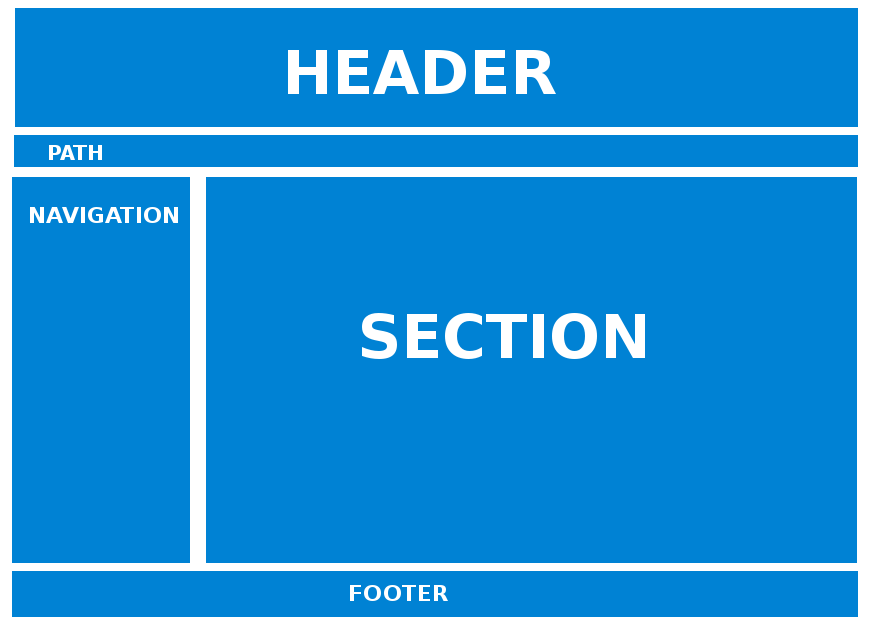
\includegraphics[scale=0.25]{layout}
\caption{Layout utilizzato dal sito}
\label{layoutPic}
\end{figure}

\begin{itemize}
 \item \textbf{Header}: parte superiore che contiene il titolo della pagina e l'indicazione della lingua.
 \item \textbf{Path}: sezione immediatamente sottostante all'header in cui viene indicata la posizione attuale assoluta all'interno del sito.
 \item \textbf{Navigation}: la parte sinistra di ogni pagina è occupata dal menù di navigazione, che contiene i link per le pagine principali.
 \item \textbf{Section}: la parte a destra del menù contiene il vero contenuto, ovvero la parte variabile che cambia per ogni pagina.
 \item \textbf{Footer}: la parte inferiore del sito contiene le informazioni accessorie, dato che è quella meno visibile per l'utente; in questo caso contiene i link ai social network, il nome team che ha realizzato il sito e le certificazioni W3C.
\end{itemize}

Per garantire una corretta visualizzazione tramite ogni dispositivo si è scelto di utilizzare un layout elastico, che permette il ridimensionamento negli schermi dei PC ma arriva ad un punto di rottura che cambia completamente la presentazione nel caso di larghezza del display troppo piccolo. In questo modo si riesce a sfruttare al meglio le diverse dimensioni, permettendone l'utilizzo sia da PC che da dispositivi mobile.
La completa divisione tra contenuto e presentazione ha reso più facile questa operazione, dato che in questo modo non è stato necessario mobificare il contenuto HTML delle pagine, ma solo il CSS.
In totale sono stati usati tre layout CSS differenti:
\begin{itemize}
 \item il principale (\textit{style.css}) contiene la presentazione per schermi medio grandi, contenente la disposizione vista precedentemente;
 \item la versione mobile per schermi piccoli (\textit{small.css}), in cui la disposizione è stata studiata per permetterne l'utilizzo tramite touchscreen, e quindi contiene bottoni più grandi ed uno stile più verticale ``scroll-friendly'';
 \item l'ultimo è il layout per la stampa (\textit{print.css}), che rimuove gli elementi che non necessitano di essere stampati (come il menù) ed utilizza un font più consono per la carta stampata (\textit{Times New Roman}).
\end{itemize}

\begin{figure}[h]
\centering
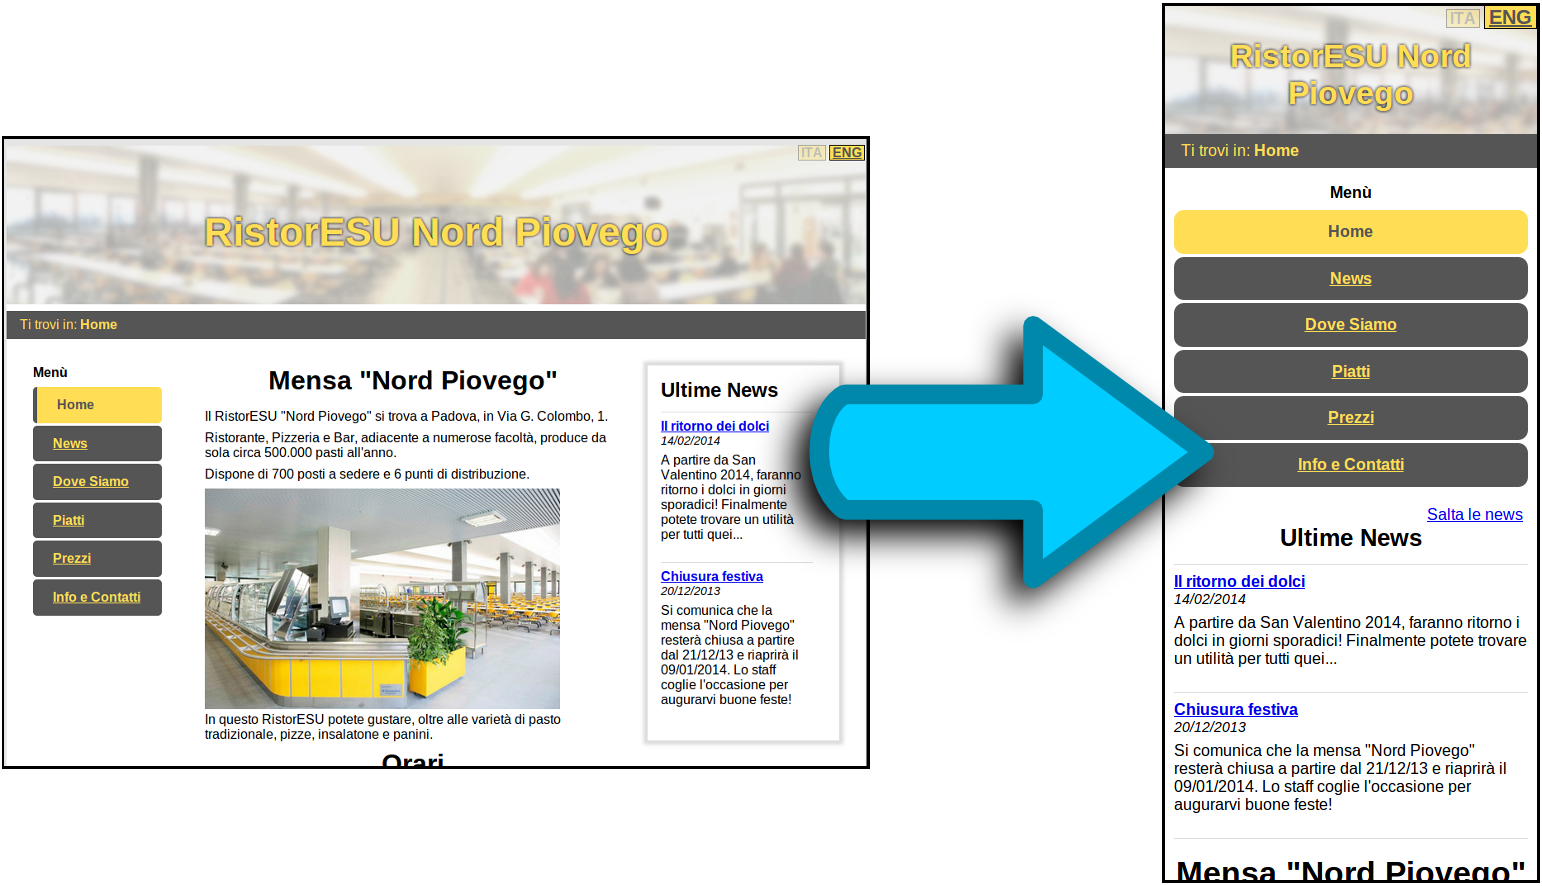
\includegraphics[scale=0.20]{trasformazione}
\caption{Layout normale e mobile}
\label{trasformazioneMobile}
\end{figure}

Inoltre, all'interno di ogni foglio di stile le dimensioni di tutti gli elementi sono state definite tramite percentuali (nel caso di posizionamenti) o ``em'' (nel caso di grandezza del testo), in modo che la pagina si adatti ad ogni tipo di schermo.
Per migliorare il supporto ai diversi sistemi operativi sono state definite più famiglie di font, in modo che l'assenza di supporto per uno specifico font non causi un fallback su un altro non adatto per il sito; in particolare, l'ordine di font family è \textit{Helvetica}, \textit{Arial} e \textit{sans-serif}.

\subsection{Struttura organizzativa}

La struttura organizzativa utilizzata dal sito è gerarchica, ed è stata scelta per permettere all'utente di orientarsi facilmente. A tale scopo è stata mantenuta una profondità media molto bassa, mantenendo anche una ridotta ampiezza utilizzando solo sei voci nel menù, in modo che l'utente possa facilmente creare una propria mappa mentale e evitare il disorientamento.
Inolte si è cercato di mantenere sempre presenti alcune informazioni importanti, che permettano di rispondere alle principali informazioni di cui l'utente ha bisogno. Per farlo è stato controllato che le sei domande principali rappresentate dai sei assi W fossero risposte nell'home page, come ad esempio ``Di cosa parla il sito?'', ``Cosa offre il sito?'', o ``Come raggiungere le sezioni principali del sito?''.

\section{Dati}

I dati del sito sono salvati in un database XML, per cui è stato definito un XMLSchema che propone la struttura visibile nella Figura \ref{xml}. È stato usato il modello di progettazione ``tende alla veneziana'', in modo da garantire la possibilità di riutilizzo dei tipi avendo solo un elemento globale. 
È stato deciso di utilizzare un solo database per tutto il sito, utilizzando di volta in volta solo alcune informazioni durante la generazione delle pagine; questa scelta è stata dettata dal fatto che tutti i dati inseriti sono logicamente correlati tra loro.
Considerando che l'elaborazione viene effettuata server side, non è presente il problema dello spreco di banda per l'invio della totalità delle informazioni, poichè al client vengono inviate solo le informazioni effettivamente visualizzate.
La radice ``piatti'' rappresenta quale tipologia di dati vogliamo salvare, cioè le informazioni relative alle portate disponibili.
Gli altri elementi importanti sono:
\begin{itemize}
 \item \textbf{Piatto}: rappresenta il singolo piatto, e contiene le informazioni principali, quali il nome, la descrizione e l'immagine (come path). Inoltre tutte le informazioni contenenti testo sono state aggiunte due volte utilizzando un suffisso diverso per il nome dell'elemento: uno per la lingua italiana e uno per la lingua inglese.
 \item \textbf{Commento}: ogni piatto contiene un figlio ``\textit{commenti}'', che a sua volta può contenere molti figli ``\textit{commento}'', che possiedono tutte le informazioni relative ad un singolo commento, come la data, l'autore, il testo e la lingua utilizzata dall'utente durante la scrittura.
\end{itemize}
Come detto precedentemente, pagine diverse utilizzano diversi elementi del database, in particolare:
\begin{itemize}
 \item il foglio di trasformazione piatti.xsl utilizza gli elementi ``\textit{piatto}'' per costruire dinamicamente la lista delle portate disponibili;
 \item il foglio viewpiatto.xsl utilizza l'elemento ``\textit{piatto}'' e le sue informazioni per costruire un resoconto dettagliato di una singola portata, includendo anche la visualizzazione dei commenti.
\end{itemize}
L'utilizzo specifico verrà trattato successivamente all'interno della descrizione delle singole pagine.

\begin{figure}[h]
\centering
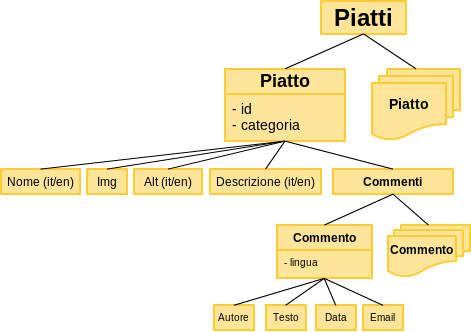
\includegraphics[scale=0.55]{alberoXML}
\caption{Struttura del file piatti.xml}
\label{xml}
\end{figure}

\section{Analisi generale dell'accessibilità}

Riguardo l'accessibilità si è scelto di rispettare le direttive WCAG 2 AAA, e alcune delle scelte più importanti verranno descritte di seguito.

\subsubsection{Colori}

Come anticipato precedentemente, la scelta cromatica è stata fatta in base ai colori che rappresentano al meglio la mensa Piovego. Prima di applicare i vari colori al sito, è stato controllato che mantenessero sempre un contrasto molto alto, in modo da non creare alcun problema di accessibilità a persone con disturbi visivi. Inoltre in tutto il sito non sono mai state veicolate informazioni tramite colori, per evitare che gli utenti ipovedenti, o con problemi di daltonismo, non riescano ad accedervi. Un esempio è la barra nera presente a fianco dell'elemento del menù selezionato, in modo che l'informazione sulla pagina corrente sia più evidente. \\
Per l'analisi in caso di daltonismo ci siamo affidati al sito \textit{http://vischeck.com/}, e i risultati sono evidenti dalla Figura \ref{colors}. Si può notare che i contenuti sono comprensibili anche nel caso più raro di tritanopia. \\

\begin{figure}[h]
\centering
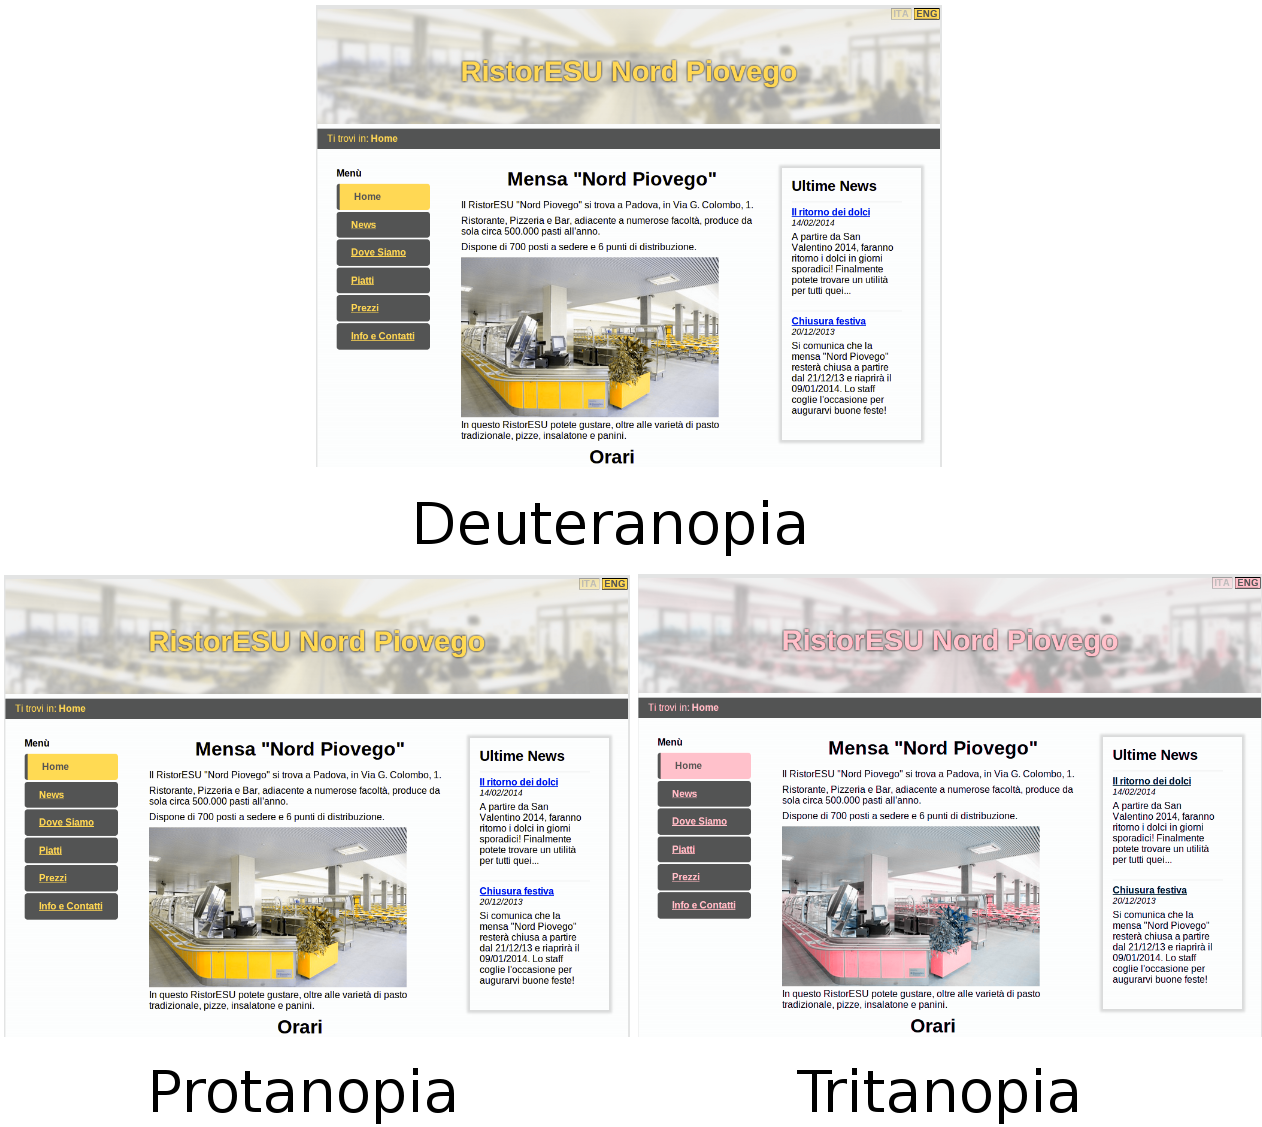
\includegraphics[scale=0.25]{home_colors}
\caption{Come viene vista l'home page in caso di daltonismo}
\label{colors}
\end{figure}

\subsubsection{Testo}

Il testo viene presentato con un font di dimensione sufficiente ad una facile lettura, anche per persone ipovedenti. Oltre a questo la dimensione del carattere è stata impostata tramite ``em'', in modo da adattare il testo in funzione delle caratteristiche preferite dall'utente.
La struttura dei paragrafi ha seguito una divisione in sezioni in modo da favorire la semplicità di lettura. In particolare in \textit{prices.html} / \textit{prices\_en.html}, poichè la quantità dei contenuti è molto elevata, il testo è stato diviso in varie sezioni raggiungibili direttamente da link posti ad inizio pagina; inoltre sono stati inseriti molti elenchi puntati, in modo tale da offrire una struttura più schematica alle informazioni presentate, aumentandone l'usabilità.

\subsubsection{Immagini}

L’uso di immagini all’interno di questo sito è avvenuto, principalmente, per due scopi:
\begin{itemize}
 \item presentazione: come per l’immagine contenuta all’interno dell’header del sito e presente in tutte le pagine. La definizione di queste immagini è avvenuta tramite assegnamento dello sfondo dell’header nel foglio di stile e non sono state aggiunte informazioni aggiuntive, in quanto elemento di sola presentazione. In particolare, il titolo ``RistorESU Nord Piovego'' presente nell’header è stato creato come semplice contenuto testuale (con successive applicazioni di stili idonei) e non come parte dell’immagine di sfondo per evitare problemi durante la fase di resize del browser o nella visualizzazione a risoluzioni diverse;
 \item contenuto: le altre immagini presenti nel sito, quali le anteprime dei piatti o le foto illustrative dell’interno della mensa, sono state definite tramite tag <img> avendo l’accortezza di inserire sempre l’attributo ``alt'' in modo da spiegarne brevemente il contenuto anche agli utenti che non possono visualizzarle.  In alcuni casi sono state anche utilizzate come collegamenti ipertestuali, come per le immagini dei piatti o i link nel footer ai social network e ai validatori.
\end{itemize}
Sempre per quanto riguarda le immagini, abbiamo cercato di mantenere una dimensione accettabile delle stesse, raggiungendo un compromesso tra buona qualità di visualizzazione e bassa occupazione di banda. Come fatto per i colori, anche per le immagini è stata fatta attenzione a mantenere sempre un contrasto elevato, in modo da agevolare la visualizzazione da parte di soggetti ipovedenti.

\subsubsection{Link}

Per migliorare l’accessibilità, tutti i link ipertestuali contenuti nel sito sono composti da testo sottolineato. Inoltre, per quanto riguarda i link del menù laterale, l’area cliccabile è stata estesa a tutta la superficie del bottone.
All’interno di questo sito si è fatto uso frequente di link per due scopi:
\begin{itemize}
 \item agevolare la navigazione interna per pagine particolarmente cariche di contenuto tramite l’utilizzo di ancore (con collegamenti del tipo ``Torna all’inizio'');
 \item fornire collegamenti a pagine esterne per il reperimento di ulteriori informazioni
\end{itemize}
In entrambi i casi, si é scelto di indicare i link visitati con un colore diverso rispetto a quello dei link non ancora visitati, rispettando così la consolidata convenzione largamente usata nelle pagine web e aiutando l’utente a ricordare la mappa corrente di navigazione (cercando di eliminare, grazie anche al breadcrumb, il problema del \textit{lost in navigation}), evitando un sovraccarico cognitivo. Un altro tipo di link utilizzato è il ``\textit{mailto}'', per consentire all’utente di inviare mail, tramite il proprio client di posta, agli indirizzi indicati per ottenere informazioni. 

\subsubsection{Screen Reader}

Il problema principale affrontato nella progettazione del sito in ambito di screen reader è stata la commutazione tra lingua italiana e inglese: le pagine in lingua inglese contengono alcune parole italiane e le pagine in lingua italiana contengono alcune parole inglesi, quindi è stato necessario aggiungere l’attributo xml:lang=``it'' (xml:lang=``en'') per permettere allo screen reader di pronunciare la parola nella lingua corretta.
Un altro accorgimento è stato introdotto nell'inserimento delle immagini: ogni immagine inserita contiene l'attributo alt, che permette allo screen reader di leggere la descrizione dell'immagine che non può essere visualizzata.
Nella home è presente una tabella che indica il menù della settimana; al fine di permettere allo screen reader di leggere la tabella e far comprenderne meglio il contenuto all'utente, è stato inserito l'attributo ``summary'' che descrive il contenuto e la struttura della tabella e l'elemento ``scope'' che, in fase di lettura, indica le intestazioni relative all'elemento che sta leggendo in quel momento.

\subsubsection{Tabindex}

In tutte le pagine web sono stati inseriti gli attributi ``tabindex'' all'interno dei link di navigazione. Utilizzando il tasto ``tab'' quindi è possibile passare da un link all'altro come se si stessero scorrendo i campi di un form. Questa modalità di selezione permette agli utenti sprovvisti di mouse (o comunque in grado di usare solo la tastiera) di selezionare correttamente tutti i link della pagina corrente.

\clearpage
\section{Mappa del sito}

\includegraphics[width=.9\textwidth]{mappasito.png}


\clearpage

\section{Pagine significative}

Verranno ora descritte le tecniche scelte ed utilizzate nella costruzione delle pagine con caratteristiche diverse rispetto al resto del sito.

\subsection{Index}

La pagina principale si propone di fornire all'utente appena arrivato le informazioni necessarie per avere una preview generale e contemporaneamente visualizzare i vari assi lungo i quali può continuare la sua navigazione interna. In particolare, per questi scopi, nella pagina principale si possono notare:
\begin{itemize}
 \item il menù a sinistra: presente in tutte le pagine, guida l'utente attraverso le sezioni del sito ovvero ``News'', ``Dove siamo'', ``Piatti'', ``Prezzi'' ed ``Info e contatti'';
 \item la sezione ``Ultime News'': fornisce all'utente le informazioni più recenti inerenti la mensa. Nella pagina principale vengono fornite solo delle anteprime brevi degli articoli o notizie, le quali possono essere lette interamente cliccando sul titolo, accedendo direttamente alla pagina delle news;
 \item un breve testo di presentazione con foto illustrativa;
 \item Un calendario con il menù della settimana. Questa è l'informazione principale che un utente solitamente cerca in un sito di questo tipo, pertanto abbiamo ritenuto opportuno includerlo nella pagina home. Con lo scopo di renderlo più usabile, si è deciso di visualizzare il giorno corrente con un colore diverso rispetto agli altri tramite javascript, come sarà descritto nella sotto-sezione seguente.
\end{itemize}
Nella pagina Index, come in tutte le altre, sono presenti i meta tag nella sezione head:
\begin{itemize}
 \item \textit{Author}: con gli autori della pagina;
 \item \textit{Description}: con una breve descrizione della pagina che si sta visitando;
 \item \textit{Keywords}: con le parole chiave inerenti la pagina, come ``ristorazione'', ``padova'' e ``studenti'';
 \item \textit{Language}: con la lingua della pagina corrente che consente allo screen reader di leggere la pagina con pronuncia corretta.
\end{itemize}
Ovviamente, i contenuti dei metatag con contenuto in italiano, sono stati tradotti per le pagine in inglese.

\subsubsection{Disposizione}

Nell'affrontare la creazione delle varie sezioni della pagina Index.html, in particolare per quanto riguarda la sezione news, si é notato che la visualizzazione finale non era indipendente dall'ordine con il quale venivano inseriti i contenuti all'interno del \textit{div} contenitore. 
Infatti, particolari ordinamenti di questi \textit{div} portavano a problemi di allineamento degli stessi, con risultati molto diversi da quanto desiderato. Nonostante questo potesse sembrare una violazione dell'indipendenza tra contenuto e presentazione, si é fatto riferimento a siti simili (come ad esempio il sito del corso di informatica dell'Universita di Padova), per trovare il giusto ordine di \textit{div} contenitori che non creasse problemi di presentazione.
Come accennato in precedenza, i link alle notizie portano alla pagina news direttamente alla notizia che si stava leggendo, tramite un'ancora passata in querystring.

\subsubsection{Javascript}

Nella pagina home, vengono utilizzati due script. Il primo è utilizzato per selezionare il giorno corrente nella tabella delle pietanze della settimana, in modo da agevolare l'utente nella ricerca di informazioni. Questo è ottenuto tramite la funzione \textit{getDay()}, con la successiva applicazione di uno stile idoneo alla riga del giorno corrente.
\begin{figure}[h]
\centering
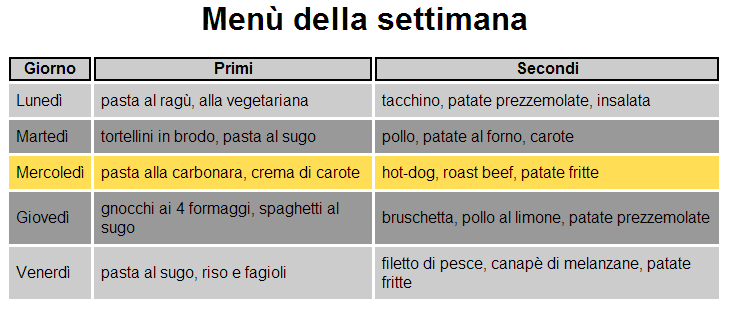
\includegraphics[scale=0.45]{tabellaMenu}
\caption{La tabella del Menù, con Mercoledì evidenziato}
\label{tabellaMenu}
\end{figure}
Il secondo, invece, effettua l'assegnazione ad ogni link a pagine esterne dell'evento \textit{onclick()} con l'apertura in una nuova tab. In linea teorica, questo si sarebbe potuto ottenere con l'assegnazione di tale evento da codice HTML ma avrebbe leso la separazione tra contenuto e comportamento. 
Entrambi gli script sono inclusi, insieme ad altre funzioni utilizzate successivamente, nel file script.js, esterno alla pagina HTML di modo da creare un ulteriore livello di separazione tra contenuto e comportamento.

\subsection{Dove Siamo}

La pagina ``Dove Siamo'' contiene le informazioni che permettono all’utente di trovare facilmente la posizione geografica della mensa. Le indicazioni sono state inserite sia in forma testuale che sotto forma di immagine, in modo da permetterne la fruizione anche da persone con problemi di vista.

\subsubsection{Mappa}

Per permettere di aumentare il grado di interazione del sito e’ stato deciso di aggiungere anche un iframe collegato alla mappa di google, in modo che sia possibile non solo sapere la posizione, ma anche calcolare il percorso per raggiungerla.
Il principale problema di questa funzione è dato dal fatto che l’introduzione di un iframe comporta possibili problemi di accessibilità e la pagina risulta non valida secondo gli standard del W3C.
Per risolvere questo problema e’ stato necessario considerare le varie situazioni di utilizzo ed utilizzare CSS e JavaScript per adattare la visualizzazione.
Nella struttura della pagina è solo presente un’immagine statica, che viene cambiata con un’altra con zoom maggiore in caso di layout mobile (tramite CSS). Questa versione basilare è valida secondo gli standard W3C. Successivamente al caricamento, uno script JavaScript aggiunge l’iframe contenente la mappa interattiva e nasconde l’immagine. In questo modo tutti i browser che supportano JavaScript potranno godere del contenuto migliorato, mentre gli altri non noteranno alcuna differenza (degrado aggraziato). Nel caso di stampa, il CSS si occupa di nascondere l’iframe e mostrare l’immagine in modo che possa essere stampata.
Nel caso in cui la pagina venga letta da uno screen reader non sono presenti problemi, dato che verrà letto l’attributo ``alt'' dell’immagine, rispettando i requisiti di accessibilità. Purtroppo non è possibile migliorare l’esperienza d’uso in questo caso, dato che la mappa interattiva è inaccessibile per definizione per utenti con problemi di vista, ma con questa soluzione evita di creare problemi.

\subsection{Piatti}

Lo scopo di questa pagina è quello di presentare all’utente la lista delle pietanze disponibili in mensa, divise per ordine di portata (primo, secondo e dessert). In particolare è stata fatta particolare attenzione al layout per la stampa di questa pagina, rimuovendo ogni link superfluo e colori di sfondo che avrebbero potuto causare un utilizzo ingiustificato di inchiostro.

\begin{figure}[h]
\centering
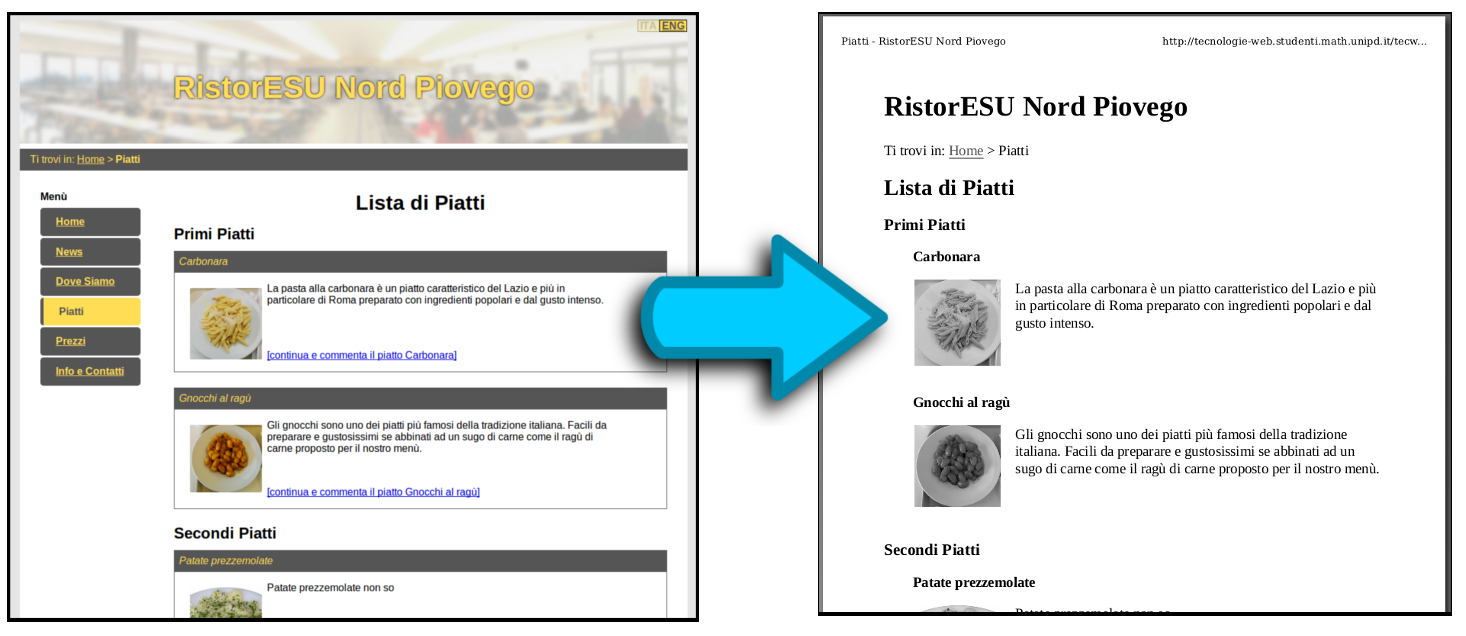
\includegraphics[scale=0.20]{trasformazioneStampa}
\caption{Layout normale e per la stampa}
\label{trasformazioneStampa}
\end{figure}

\subsubsection{Creazione dinamica}

L’elenco dei piatti è memorizzato all’interno del file \textit{piatti.xml}. Per poterli presentare all’utente è stato creato un foglio di trasformazione di stile \textit{piatti.xsl} che è in grado di estrarre dall’intero database solo le informazioni di cui ha bisogno, scartando quindi i commenti, i nomi e le descrizioni scritte in lingua diversa da quella correntemente selezionata.
Per presentare queste informazioni all’utente vengono create tre differenti DefinitionList, una diversa per ogni tipo di categoria presente (Primi Piatti, Secondi Piatti e Desserts).
Per ogni categoria viene effettuato un xsl:for-each sui nodi <piatto>, facendo una selezione sull’attributo @categoria. Per ogni piatto viene creato un DefinitionTitle con il nome del piatto corrente, e un corrispondente DefinitionDescription con immagine, descrizione e link alla pagina specifica in cui è possibile inserire e leggere i commenti.
L’applicazione del foglio di trasformazione di stile al database XML viene effettuata lato server per diversi motivi, principalmente per alleggerire il carico di banda all’utente che vuole visualizzare la pagina. Facendo effettuare la trasformazione in locale al browser dell’utente, sarebbe stato necessario scaricare l’intero database, comprensivo dei commenti per ogni piatto, mostrandone però solo una minima parte. Inoltre alcuni browser (come ad esempio quelli testuali) non sono in grado di effettuare tale trasformazione. Facendo la trasformazione in locale inoltre gli utilizzatori di dispositivi mobile avrebbero sofferto un notevole calo delle prestazioni visitando la pagina, in quanto l’elaborazione è una operazione computazionalmente molto costosa.
La trasformazione lato server viene effettuata utilizzando la libreria XML::LibXSLT, che consente di applicare il foglio di trasformazione direttamente all’XML dopo una fase di parsing per controllare che siano entrambi ben formati.
E vero che questa scelta potrebbe causare un carico di lavoro eccessivo lato server, ma considerando le alternative è sembrata la scelta piu ragionevole, specialmente considerando il fatto che utilizzando tecniche di caching sarebbe possibile minimizzare tale carico.
In questo caso la traduzione in differenti lingue è stata effettuata selezionando quale foglio di trasformazione utilizzare tramite il valore del parametro lang passato in GET nell’URL della pagina.

\subsection{Viewpiatto}

La pagina viewpiatto, accessibile dalla lista dei piatti, permette di ottenere informazioni dettagliate riguardo una pietanza. Il contenuto è totalmente incentrato sul singolo piatto, e comprende il nome, l’immagine e la descrizione. Più in basso sono presenti i commenti precedentemente inviati dagli utenti, e nella parte finale è presente un form che consente l’invio dei commenti.
Essendo l’unica pagina di secondo livello, il menù non contiene alcun elemento selezionato, e la path indica il percorso corrente.

\subsubsection{Creazione dinamica}

Per evitare di dover creare una pagina per ogni pietanza, è stato deciso di scrivere una pagina dinamica, che adatti il contenuto all’id del piatto.
La generazione della pagina è divisa in due parti, la selezione del nodo tramite Perl, e la trasformazione da XML ad XHTML tramite XSLT.
Per la prima parte viene utilizzato Perl ed il modulo CGI, che agevola la lettura dei parametri; dalla lista dei piatti viene passato alla nuova pagina l’ID del piatto richiesto e la lingua. Una volta letti, lo script ha il compito di trovare il nodo ``piatto'' nell’XML, tramite XPATH.
A questo punto, tramite la libreria LibXSLT il nodo viene trasformato mediante il foglio di stile viewpiatto.xsl, in modo da ottenere la pagina XHTML da inviare al client. Anche in questo caso la lingua è stata scelta in base al parametro lang inviato precedentemente.
L’invio dei parametri è stato effettuato tramite GET, e quindi con i valori visibili nell’URL; questa scelta si è basata sulla possibilità di permettere il salvataggio della pagina come bookmark, cosa non possibile se si fosse usato POST. Inoltre i dati visibili nell’URL sono l’ID e la lingua, ossia solo informazioni non sensibili.

\subsubsection{Form}

Il form è la parte della pagina che permette l’interazione da parte dell’utente. In questo caso consente l’inserimento di commenti relativi al piatto visualizzato.
Le informazioni richieste all’utente sono il nome, la mail ed il testo del commento.
Per garantire una buona accessibilità, ogni voce del form è identificata da una label chiara, ed i vari campi sono raggiungibili anche tramite tabindex.

\subsubsection*{Client}

Per diminuire il carico di lavoro per il server si è deciso di aggiungere i controlli di inserimento dei dati tramite JavaScript (non sostitutivi ai controlli server side), in modo da avere un resoconto immediato su eventuali campi compilati in modo non corretto. Ad ogni perdita di focus di un campo viene controllato che il contenuto rispetti alcuni canoni, come la lunghezza minima e massima del campo nome e commento, o il pattern della mail.
Anche alla pressione del bottone di invio ogni campo viene controllato nuovamente, e in caso almeno uno dei box contenga errori l’invio viene bloccato, e quindi viene evitato lo spreco di banda per la restituzione dell’errore. In caso non siano presenti errori, il pulsante di invio viene disabilitato subito dopo il click, in modo da dare il tempo allo script lato server di prendere in carico la richiesta e di reindirizzare l’utente alla nuova pagina contenente il commento appena inserito, evitando accidentali invii multipli.
Inoltre sono stati aggiunti campi aggiuntivi rispetto a quelli visibili dall’utente, che permettono di comunicare alcune informazioni che sono implicite nella pagina, come la lingua e l’ID del piatto.

\subsubsection*{Server}

Lo script perl a cui si interfaccia il form è \textit{insertComment.cgi}, che si occupa di ricevere i parametri inviati in POST e di aggiungere le nuove informazioni al database attuale.
Prima di inserire i dati nel database, viene effettuato un processing per evitare ad un utente malevolo la possibilità di corrompere il file XML in cui sono salvate le informazioni.
Per ogni parametro ricevuto vengono ripetuti i controlli effettuati da javascript, in modo da poter controllare anche gli utenti che non lo hanno abilitato o che non hanno buone intenzioni. In particolare il controllo di validità dell’indirizzo e-mail viene effettuato utilizzando la libreria Email::Valid, mentre la lunghezza dei campi nome e descrizione viene valutato con la funzione length().
Prima di inserire i dati vengono eliminati alcuni caratteri speciali che potrebbero danneggiare la struttura del file, quali <, > e \&. Questi caratteri vengono sostituiti da un *, in modo da non impattare sulla lunghezza effettiva del nome/commento.
Per evitare problemi che potrebbero sorgere a causa di un accesso concorrente in scrittura da parte di due client differenti, viene aperto un file di lock e usata la funzione flock() con parametro LOCK\_EX, che resta in attesa finchè non riesce effettivamente ad ottenere il lock esclusivo.
Prima di rilasciare il lock, viene letto lo stato attuale del database, aggiunti i nuovi dati creando un nodo figlio nella posizione corretta, e scritto il nuovo file aggiornando il database. All’interno del nuovo nodo creato vengono inseriti gli attributi di lingua, che serviranno alla pagina di visualizzazione per inserire correttamente gli attributi xml:lang per gli screen reader.

\clearpage

\section{Test}

Sono stati provati i seguenti browser su sistemi operativi Windows e Linux, sia con aspect ratio 16:9 che 4:3:
\begin{itemize}
 \item Chrome 33
 \item Firefox 23 e 28
 \item Internet Explorer 11
 \item Opera 12.16
 \item Steam Browser
 \item Konqueror 4.8.5
\end{itemize}
I test su dispositivi mobile sono stati effettuati tramite:
\begin{itemize}
 \item Tablet:
 \begin{itemize}
  \item Internet Explorer 11 (versione touch)
  \item Safari su iPad (iOS 7)
 \end{itemize}
 \item Smartphone:
 \begin{itemize}
  \item Chrome 33, Xperia Browser, e Default Browser su Android
  \item Safari su iPhone (iOS 7)
 \end{itemize}
\end{itemize}
Su Mac sono stati provati:
\begin{itemize}
 \item Safari 7
 \item Chrome 33
 \item Firefox 
\end{itemize}
Su tali browser non è stata riscontrata nessuna problematica di sorta. \\
I test con:
\begin{itemize}
 \item Internet Explorer 7 e 8
 \item Kindle Touch
\end{itemize}
hanno evidenziato qualche problema nell’interpretare alcune istruzioni CSS3, come ad esempio il text-shadow per il titolo nell’header e il border-radius per alcuni elementi del layout.
Questo ha danneggiato lievemente la leggibilità del titolo nell’header, ma considerando che si tratta di un elemento presentazionale e non di contenuto si è preferito non utilizzare tecniche di code-forking per utilizzare soluzioni alternative in caso di assenza di text-shadow.
In generale il sito rimane utilizzabile e i contenuti restano fruibili.
Inoltre da IE 8 in giù la mancanza del supporto a CSS3 non permette di differenziare il colore delle righe nella tabella nella home. Il risultato è leggermente meno leggibile (il diverso colore aiuta ad identificare le righe), ma non causa problemi di accessibilità.
Sono stati testati i due browser testuali Lynx e Links, e neppure qui sono stati riscontrati problemi di accessibilità: i collegamenti sono tutti visibili e ogni immagine che non può essere visualizzata è stata sostituita con un testo descrittivo. Anche le pagine \textit{.cgi} funzionano correttamente, compreso il form per i commenti.
L'ultimo test è stato effettuato su un simulatore di sceen reader: la struttura del sito e i link visibili solo da questi dispositivi hanno reso accessibile e facilmente fruibile i contenuti proposti.

\section{Validazione}

Tutte le pagine sono state verificate secondo gli standard del W3C, verificando tramite il sito \textit{http://validator.w3.org/} e \textit{http://jigsaw.w3.org/css-validator/} che sia l’XHTML che il CSS fossero validi (come confermato dal logo nel footer di ogni pagina).
Inoltre, utilizzando il software Total Validator è stato verificato che il sito rispetti le linee guida proposte dal WCAG, riuscendo ad ottenere la conformità al livello AAA riguardo l’accessibilità.

\section{Conclusioni}

Lo scopo di questo progetto vuole essere il mostrare una “demo” di un sito, rispettando requisiti di accessibilità. Alcune funzionalità sarebbero necessarie nella versione “completa” del sito, ma non sono state effettivamente realizzate poichè non ritenute necessarie ai  fini del corso.
Serve ad esempio una pagina di amministrazione, che consenta di moderare i commenti inseriti (dando la possibilità di rimuoverli), aggiungere/rimuovere/modificare nuovi piatti o aggiungere le news. Inoltre sarebbe necessario chiedere una conferma via mail prima della pubblicazione del commento, il che sarebbe stato possibile tramite Perl se non fosse che l’invio di messaggi e-mail dal server del corso è stato bloccato per ovvi motivi di sicurezza.

\end{document}


